\newpage
\section{Architektura systemu}

System opiera się na dwóch rodzajach agentów
\begin{itemize}
\item kierowców samochodów z zainstalowaną aplikacją
\item parkingów agregujących miejsca parkingowe
\end{itemize}

Celem kierowców jest znalezienie parkingu jak najbliżej aktualnego miejsca.
Celem parkingów jest zapełnienie się i zadowolenie kierowcy. Kierowca może wybrać jeden spośród proponowanych parkingów i podążać do niego.

System wymaga, aby samochód cyklicznie wysyłał zapytania do parkingów otrzymując w odpowiedzi ich położenie. 

System uzgadniania miejsc nie może dopuścić do sytuacji gdy przy jednoczesnym zgłoszeniu chęci parkowania przez dwa lub więcej samochody zostaną przydzielone dwa samochody na jedno wolne miejsce parkingowe.

Parking nadzoruje, czy kierowca nie oddala się od niego po zgłoszeniu chęci zaparkowania przez dłuższy czas lub nie wysłał zgłoszenia dotyczącego anulowania rezerwacji. W przypadku wystąpienia jednego z tych zdarzeń parking odwołuje rezerwację zwalniając przydzielone dla samochodu miejsce.

Miejsca parkingowe są natomiast aktorami będącymi nieaktywnymi przez większość czasu. Ich zadanie polega jedynie na wysyłaniu komunikatów do parkingu, do którego przynależą. Jest to komunikat o zajęciu i zwolnieniu miejsca przez kierowcę. Na tej podstawie parking wie ile samochodów znajduje się na nim, a ile może przyjąć. Od liczby samochodów, które parking może przyjąć należy odjąć również samochody, które zgłosiły chęć parkowania, ale jeszcze nie dojechały. Nigdy jednak nie zostaje przyjęte więcej samochodów niż liczba wolnych miejsc.

Kierowcy komunikują się z parkingami zgłaszając chęć parkowania lub odrzucając sugerowany parking. Generalnie nie ma potrzeby, aby samochody prowadziły komunikację między sobą.


\begin{figure}[H]
    \label{fig:architektura}
    \centering 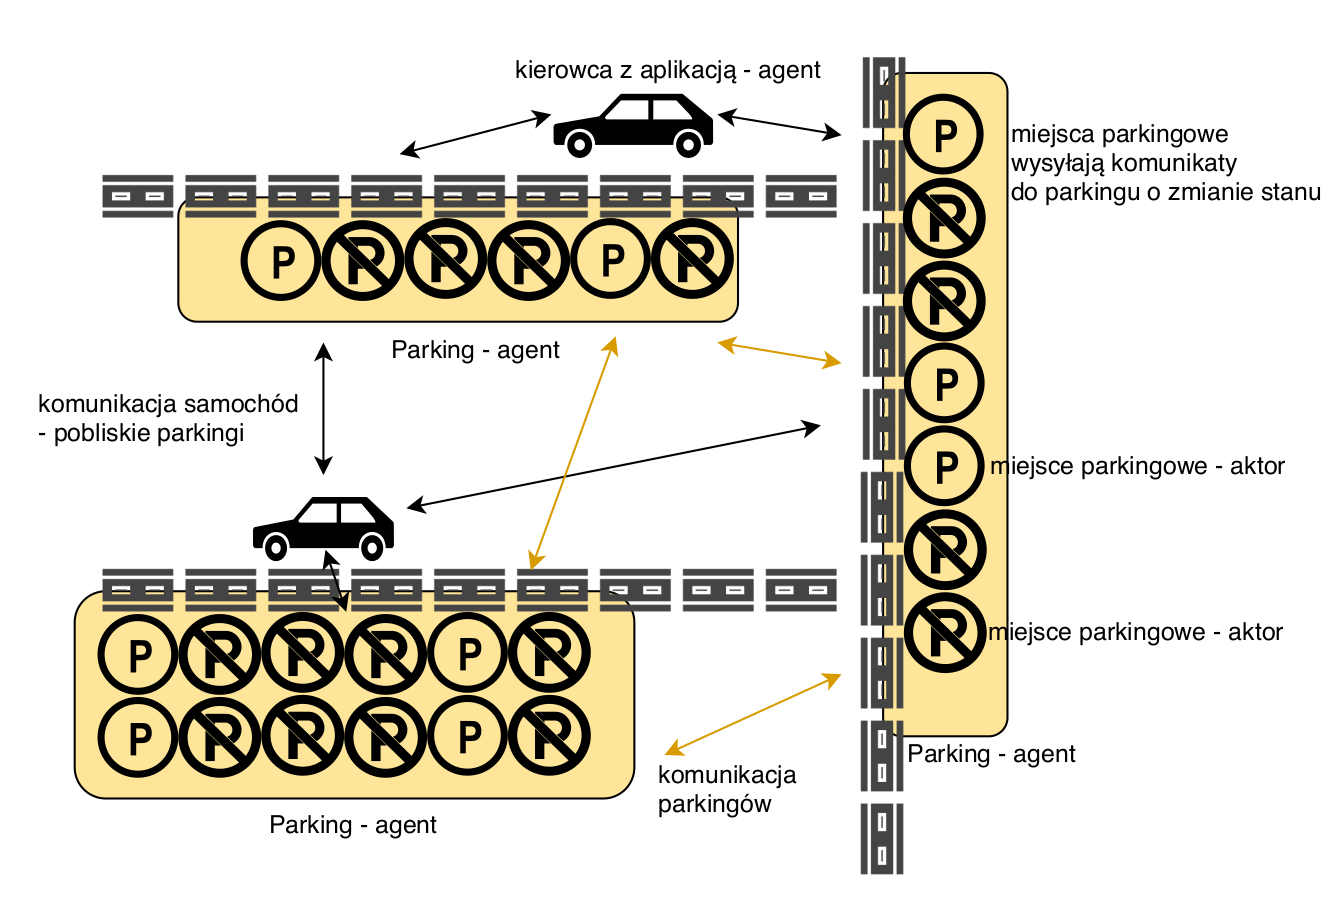
\includegraphics[width=1.1\linewidth]{archi.png}
    \caption{Architektura systemu.}
\end{figure}